\documentclass{article}

\usepackage{fancyhdr}
\usepackage{lastpage}
\usepackage{extramarks}
\usepackage[usenames,dvipsnames]{color}
\usepackage{courier}
\usepackage{amsmath}
\usepackage{amsthm}
\usepackage{amsfonts}
\usepackage{tikz}

\usetikzlibrary{automata,positioning}

\topmargin=-0.45in
\evensidemargin=0in
\oddsidemargin=0in
\textwidth=6.5in
\textheight=9.0in
\headsep=0.25in

\linespread{1.1}

\pagestyle{fancy}
\lhead{\hmwkAuthorName}
\chead{\hmwkClass\ (\hmwkClassInstructor\ \hmwkClassTime): \hmwkTitle}
\rhead{\firstxmark}
\lfoot{\lastxmark}
\cfoot{}
\renewcommand\headrulewidth{0.4pt}
\renewcommand\footrulewidth{0.4pt}

\setlength\parindent{0pt}

\newcommand{\enterProblemHeader}[1]{
    \nobreak\extramarks{#1}{#1 continued on next page\ldots}\nobreak
    \nobreak\extramarks{#1 (continued)}{#1 continued on next page\ldots}\nobreak
}

\newcommand{\exitProblemHeader}[1]{
    \nobreak\extramarks{#1 (continued)}{#1 continued on next page\ldots}\nobreak
    \nobreak\extramarks{#1}{}\nobreak
}

\setcounter{secnumdepth}{0}
\newcounter{homeworkProblemCounter}

\newcommand{\homeworkProblemName}{}
\newenvironment{homeworkProblem}[1][Problem \arabic{homeworkProblemCounter}]{
    \stepcounter{homeworkProblemCounter}
    \renewcommand{\homeworkProblemName}{#1}
    \section{\homeworkProblemName}
    \enterProblemHeader{\homeworkProblemName}
}{
    \exitProblemHeader{\homeworkProblemName}
}

\newcommand{\problemAnswer}[1]{
    \noindent\framebox[\columnwidth][c]{\begin{minipage}{0.98\columnwidth}#1\end{minipage}}
}

\newcommand{\homeworkSectionName}{}
\newenvironment{homeworkSection}[1]{
    \renewcommand{\homeworkSectionName}{#1}
    \subsection{\homeworkSectionName}
    \enterProblemHeader{\homeworkProblemName\ [\homeworkSectionName]}
}{
    \enterProblemHeader{\homeworkProblemName}
}

\newcommand{\hmwkTitle}{Homework\ \#4}
\newcommand{\hmwkDueDate}{February 28, 2013 at 11:59pm}
\newcommand{\hmwkClass}{CS331}
\newcommand{\hmwkClassTime}{9:00am}
\newcommand{\hmwkClassInstructor}{Professor Zhang}
\newcommand{\hmwkAuthorName}{Josh Davis}

\title{
    \vspace{2in}
    \textmd{\textbf{\hmwkClass:\ \hmwkTitle}}\\
    \normalsize\vspace{0.1in}\small{Due\ on\ \hmwkDueDate}\\
    \vspace{0.1in}\large{\textit{\hmwkClassInstructor\ \hmwkClassTime}}
    \vspace{3in}
}

\author{\textbf{\hmwkAuthorName}}
\date{}

\begin{document}

\maketitle

\pagebreak

\begin{homeworkProblem}
    Find a CFG to describe \(L\).
    \\

    The CFG, \(G\), that describes \(L\) is below:

    \[
        G = (V, \Sigma, R, S)
    \]

    such that

    \[
        G = (\{A, B\}, \{a, b, c\}, R, A)
    \]
    where

    \[
        \begin{split}
            R: &
            \\
               & A \rightarrow aAc | B | \epsilon
            \\
               & B \rightarrow bB | \epsilon
        \end{split}
    \]

    \begin{figure}[here]
        \centering
        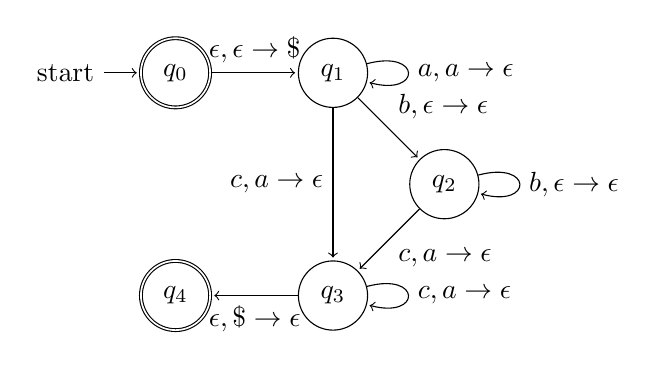
\begin{tikzpicture}[shorten >=1pt,node distance=2cm,on grid,auto] 
            \node[state, initial, accepting] (q_0) {$q_0$}; 
            \node[state] (q_1) [right=of q_0] {$q_1$}; 
            \node[state] (q_2) [below right=of q_1] {$q_2$}; 
            \node[state] (q_3) [below left=of q_2] {$q_3$}; 
            \node[state, accepting] (q_4) [left=of q_3] {$q_4$}; 
            \path[->] 
                (q_0)
                    edge node {$\epsilon, \epsilon \rightarrow \$ $} (q_1)
                (q_1)
                    edge [loop right] node {$a, a \rightarrow \epsilon $} (q_1)
                    edge node [left] {$c, a \rightarrow \epsilon $} (q_3)
                    edge node {$ b, \epsilon \rightarrow \epsilon $} (q_2)
                (q_2)
                    edge [loop right] node {$b, \epsilon \rightarrow \epsilon $} (q_2)
                    edge node {$ c, a \rightarrow \epsilon $} (q_3)
                (q_3)
                    edge [loop right] node {$c, a \rightarrow \epsilon $} (q_2)
                    edge node {$\epsilon, \$ \rightarrow \epsilon $} (q_4)
                    ;
        \end{tikzpicture}
        \caption{PDA, \(A\)}
        \label{fig:automataA}
    \end{figure}

\end{homeworkProblem}

\pagebreak

\begin{homeworkProblem}
    \textbf{Part A}
    \\
    Prove that if \(L\) is context-free and \(L'\) is a regular languagte, then
    \(L \cap L'\) is context-free too.
    \\
    
    \begin{proof}
        If \(L\) is a context-free language, and \(L'\) is a regular language, then
        let \(M\) and \(N\) be the finite automata and push down automata that
        accept both languages respectively.
        \\

        We can construct a new push down automata, \(O\) such that \(M\) and
        \(N\) both receive the input and the new machine accepts a word only if
        both \(M\) and \(N\) accept it. This is possible because a finite
        automata doesn't use a stack which means one stack is sufficient for
        the complete push down automata. This concludes the proof.
    \end{proof}

    \textbf{Part B}
    \\
    Let \(\Sigma = \{a, b, c\}\) and
    \[
        L = \{ w \in \Sigma^* | w \mbox{ contains equal number of a's, b's, and c's} \}
    \]

    Prove that \(L\) is not a context-free language.

    \begin{proof}
        Suppose \(L\) is context-free. Let \(L' = \{a^* b^* c^*\}\), a regular language.
        \\

        Then according to what we proved in the first part, \(L \cap L'\) is
        context-free. This is a contradiction because the language \(\{a^n b^n
        c^n\}\) is not context-free thus violating our previous proof. We have
        arrived at a contradiction therefore our proof is complete.

    \end{proof}

\end{homeworkProblem}

\pagebreak

\begin{homeworkProblem}
    Prove that right linear grammars recognize exactly the class of regular languages.

    \begin{proof}
        This proof will consist of two parts. First proving that any regular
        language can be described by a RLG, and that any language described by
        an RLG is regular.

        \textbf{Part One}
        Proving that any regular language can be described by an RLG.
        \\

        

        \textbf{Part Two}
        Proving that any language described by an RLG is regular.
        \\


        Since both sides have been proven, the proof is complete and RLGs
        recognize exactly the class of regular languages.

    \end{proof}
\end{homeworkProblem}

\pagebreak

\begin{homeworkProblem}
    Let \(k > 1\), \(L_k = \{\epsilon, a, aa, \dots, a^{k - 2}\}\)
    \begin{proof}
        \textbf{Part 1}
        \\

        \(L_k\) can be recognized by a DFA with k states. To show this, we will
        construct a DFA as follows:

        \begin{figure}[here]
            \centering
            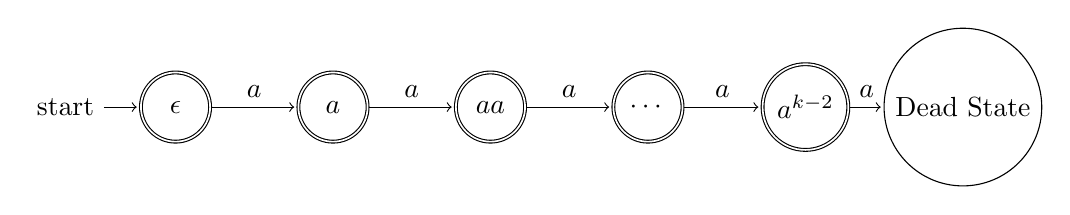
\begin{tikzpicture}[shorten >=1pt,node distance=2cm,on grid,auto] 
                \node[state, initial, accepting] (a_0) {$\epsilon$}; 
                \node[state, accepting] (a) [right=of a_0] {$a$}; 
                \node[state, accepting] (aa) [right=of a] {$aa$}; 
                \node[state, accepting] (a_dots) [right=of aa] {$\cdots$}; 
                \node[state, accepting] (a_{k-2}) [right=of a_dots] {$a^{k-2}$}; 
                \node[state] (dead) [right=of a_{k-2}] {Dead State}; 
                \path[->] 
                    (a_0)
                        edge node {$a$} (a)
                    (a)
                        edge node {$a$} (aa)
                    (aa)
                        edge node {$a$} (a_dots)
                    (a_dots)
                        edge node {$a$} (a_{k-2})
                    (a_{k-2})
                        edge node {$a$} (dead);
            \end{tikzpicture}
            \caption{DFA, \(A\)}
            \label{fig:automataA}
        \end{figure}

        As we can see, there will be one starting state, \(k-2\) additional
        states, and then one dead state. Therefore there are \(1 + (k-2) + 1 = k\) states.
    \end{proof}

    \begin{proof}
        \textbf{Part 2}
        \\
        
        We will prove by contradiction that \(L_k\) cannot be recognized by any DFA with
        \(k-1\) states.
        \\

        Assume that there is a DFA \(A\) with \(k-1\) states that accepts \(L_k\).
        \\
        
        Let \(w = a^{k-1}\) and therefore \(\left|w\right| = k - 1\). According to the definition, \(w \in L_k\). Let
        the run of \(A\) over \(w\) be \(\rho\). Thus:
        \[
            \begin{split}
                \left|\rho\right| &= \left|w\right| + 1
                \\
                &= k - 1 + 1
                \\
                &= k
            \end{split}
        \]

        Thus according to the pigeonhole principle, the number of states
        reached is equal to \(k\) yet the number of states in \(A\) is only
        \(k - 1\). That means that there exists one state in \(A\) that is visited
        twice. Let's let that state be \(q\).
        \\

        Therefore there exists a \(w'\) such that \(w' \in L_k\) and the run of
        \(A\) over \(w'\) is \(\rho' = q_0 \dots q \dots q \dots q_k\). This is true
        because if a state is visited more than once, there is a loop in \(A\)
        and \(q\) can be visited more than once
        \\

        This is a contradiction because
        \[
            \begin{split}
                \left|w'\right| &\geq \left|w\right| + 1
                \\
                &= (k - 1) + 1
                \\
                &= k
            \end{split}
        \]
        yet the largest string in \(L_k\) has length \(k - 1\) according to the
        definition of \(L_k\). Therefore we have shown that \(L_k\) cannot be
        recognized by any DFA with \(k-1\) states.

    \end{proof}
\end{homeworkProblem}

\pagebreak

\begin{homeworkProblem}
    Let \(L_n\) be the language that "the n-th letter of w from the end is 1"
    for \(n \geq 1\).

    \begin{proof}
        \textbf{Part 1}
        \\

        \(L_n\) can be recognized by a NFA with \(n + 1\) states. To show this,
        we will construct a NFA as such:

        \begin{figure}[here]
            \centering
            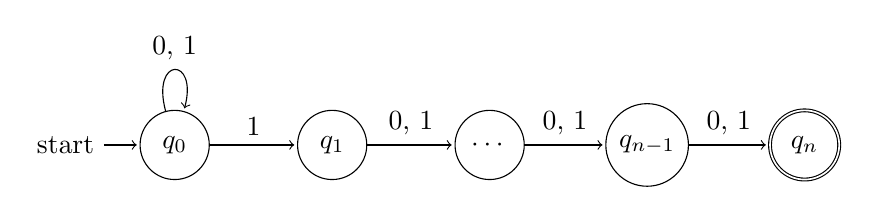
\begin{tikzpicture}[shorten >=1pt,node distance=2cm,on grid,auto] 
                \node[state, initial] (q_0) {$q_0$}; 
                \node[state] (q_1) [right=of q_0] {$q_1$}; 
                \node[state] (q_dots) [right=of q_1] {$\cdots$}; 
                \node[state] (q_{n-1}) [right=of q_dots] {$q_{n-1}$}; 
                \node[state, accepting] (q_n) [right=of q_{n-1}] {$q_n$}; 
                \path[->] 
                    (q_0)
                        edge [loop above] node {0, 1} (q_1)
                        edge node {1} (q_1)
                    (q_1)
                        edge node {0, 1} (q_dots)
                    (q_dots)
                        edge node {0, 1} (q_{n-1})
                    (q_{n-1})
                        edge node {0, 1} (q_n);
            \end{tikzpicture}
            \caption{NFA, \(A\)}
            \label{fig:automataNFA}
        \end{figure}

        As we can see, there will be one state that accepts both 0s and 1s,
        since it is an NFA we can nondeterministically skip to when the nth
        spot of a word is 1 and accept it. We can also see that to do so it
        requires one initial state, and then \(n\) states to transition through
        once there is a 1 in the nth spot. Therefore the number of states = \(n + 1\).

    \end{proof}

    \begin{proof}
        \textbf{Part 2}
        \\
        
        We will prove that any DFA that recognizes \(L_n\) needs at least \(2^n\).

        Assume there is a DFA, \(A\) with less than \(2^n\) states that accepts \(L_n\).
        Let \(A = (Q, \Sigma, \delta, q_0, F)\).
        \\

        The number of strings when we have \(n\) is equal to \(2^n\) since our
        alphabet is binary.
        \\

        Since there are \(2^n - 1\) states yet \(2^n\) strings, there must be
        two strings (according to the pigeonhole principle) such that they end
        on the same state. Or more formally \(\delta(q_0, w) = \delta(q_0, w')\).
        \\

        Since \(w, w'\) are the same length, there must be a point in each
        string where they differ from each other. Because of this, \(A\) cannot
        accept both \(w, w'\).
        \\

        Similar to problem 4, continuing this gives us a contradiction because either
        \(A\) accepts both words or it rejects both.

    \end{proof}
\end{homeworkProblem}

\end{document}
